\section{Removing disparate impact}
\label{sec:repairing-data}

Once Bob's certification procedure has made a determination of (potential) disparate impact on $D$, Alice might request a \emph{repaired} version $\bar{D}$ of $D$, where any attributes in $D$ that could be used to predict $X$ have been changed so that $\bar{D}$ would be certified as $\epsilon$-fair.  % Recall that $D = (X, Y, C) \in R^d$, where $X$ is some protected attribute, $C$ is the class outcome, and $Y$ is the set of remaining attributes. 
We now describe how to construct such a set  $\bar{D} = (X, \bar{Y}, C)$ such that $\bar{D}$ does not have disparate impact in terms of protected attribute $X$.  While for notational simplicity we will assume that $X$ is used directly in what follows, in practice the attribute used to stratify the data for repair need not directly be the protected attribute or even a single protected attribute.  In the case of the Texas Top 10\% Rule that admits the top ten percent of every high school class in Texas to the University of Texas \cite{Texas97Top10Percent}, the attribute used to stratify is the high school attended, which is an attribute that correlates with race.  
If repair of multiple protected attributes is desired, the joint distribution can be used to stratify the data.  (We will look into the effects of this experimentally in Section \ref{sec:fairness_utility}.)


Of course, it is important to change the data in such a way that predicting the class is still possible.  Specifically, our goal will be to preserve the relative per-attribute ordering as follows.  Given protected attribute $X$ and a \emph{single} numerical attribute $Y$, let $Y_x = \Pr(Y|X = x)$ denote the marginal distribution on $Y$ conditioned on $X = x$.  Let $F_x: Y_x \to [0,1]$ be the cumulative distribution function for values $y \in Y_x$ and let $F^{-1}_x: [0,1] \to Y_x$ be the associated quantile function (i.e $F^{-1}_x(1/2)$ is the value of $y$ such that $\Pr(Y \ge y|X = x) = 1/2$).
We will say that $F_x$ \emph{ranks} the values of $Y_x$.

Let $\bar{Y}$ be the repaired version of $Y$ in $\bar{D}$.  We will say that $\bar{D}$ \emph{strongly preserves rank} if for any $y \in Y_x$ and $x \in X$, its ``repaired'' counterpart $\bar{y} \in \bar{Y}_x$ has $F_x(y) = F_x(\bar{y})$. Strongly preserving rank in this way, despite changing the true values of $Y$, appears to allow Alice's algorithm to continue choosing stronger (higher ranked) applicants over weaker ones. We present experimental evidence for this in Section~\ref{sec:experiments}.

With this motivation, we now give a repair algorithm that strongly preserves rank and ensures that $\bar{D} = (X, \bar{Y}, C)$ is fair (i.e., is $\epsilon$-fair for $\epsilon = 1/2$).  In the discussion that follows, for the sake of clarity we will treat $Y$ as a single attribute over a totally-ordered domain. To handle multiple totally-ordered  attributes $Y_1, \ldots, Y_k$ we will repair each attribute individually. 

We define a ``median'' distribution $A$ 
in terms of its quantile function $F^{-1}_A$:   $F_A^{-1}(u) = \text{median\ }_{x \in X} F_x^{-1}(u)$.
The choice of the term ``median'' is not accidental. 
\begin{lemma}
\label{lemma:remov-disp-impact}
  Let $A$ be a distribution such that $ F_A^{-1}(u) = \text{median\ }_{x \in X} F_x^{-1}(u)$.
Then $A$ is also the distribution minimizing $\sum_{x \in X} d(Y_x, C)$ over all distributions $C$, where $d(\cdot, \cdot)$ is the earthmover distance on $\reals$. 
\end{lemma}
\begin{proof}
For any two distributions $P$ and $Q$ on the line, the earthmover distance (using the underlying Euclidean distance $d(x,y) = |x-y|$ as the metric) can be written as 
\[ d(P, Q) = \int_0^1 |F^{-1}_P(u) - F^{-1}_Q(u)| du \]
In other words, the map $P \mapsto F^{-1}_P$ is an isometric embedding of the earthmover distance into $\ell_1$. 

Consider now a set of points $p_1, \ldots, p_n  \in \ell_1$. Their $1$-median -- the point minimizing $\sum_i \|p_i - c\|_1$ -- is the point whose $j^{\text{th}}$ coordinate is the median of the $j^{\text{th}}$ coordinates of the $p_i$. This is precisely the definition of the distribution $A$ (in terms of $F^{-1}_A$). 
\end{proof}

\mypara{Algorithm.} Our repair algorithm creates $\bar{Y}$, such that for all $y \in Y_x$, the corresponding $\bar{y} = F_A^{-1}(F_x(y))$.  The resulting $\bar{D} = (X, \bar{Y}, C)$ changes only $Y$ while the protected attribute and class remain the same as in the original data, thus preserving the ability to predict the class.  See Figure \ref{fig:repair} for an example.

\begin{figure}[tb]
\begin{center}
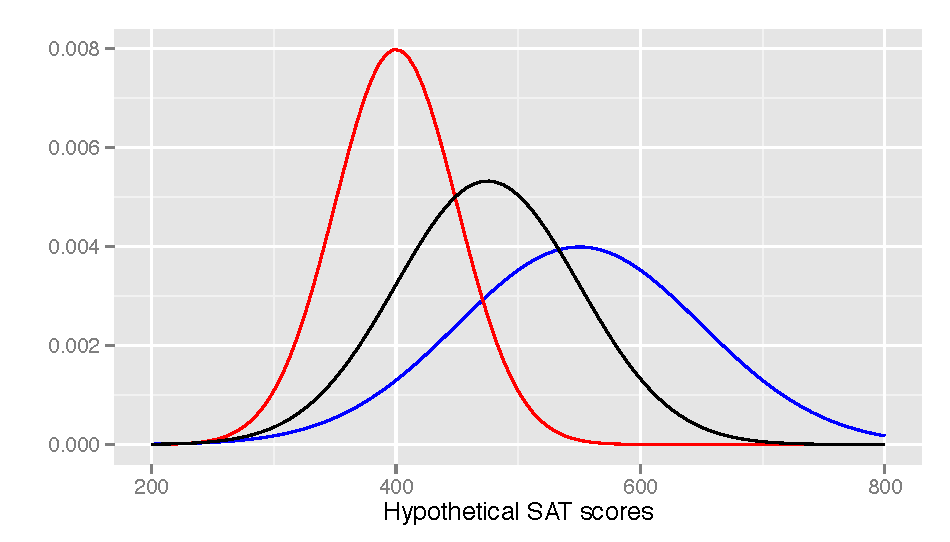
\includegraphics[width=0.75\linewidth]{fake_sat_data.pdf}
\caption{Consider the fake probability density functions shown here where the blue curve shows the distribution of SAT scores ($Y$) for $X = \texttt{female}$, with $\mu = 550,\sigma = 100$, while the red curve shows the distribution of SAT scores for $X = \texttt{male}$, with $\mu = 400,\sigma = 50$.  The resulting fully repaired data is the distribution in black, with $\mu = 475,\sigma = 75$.  Male students who originally had scores in the 95th percentile, i.e., had scores of 500, are given scores of 625 in the 95th percentile of the new distribution in $\bar{Y}$, while women with scores of 625 in $\bar{Y}$ originally had scores of 750.}
\label{fig:repair}
\end{center}
\end{figure}

\mypara{Notes.}
\label{sec:notes-1}
We note that this definition is reminiscent of the method by which partial rankings are combined to form a total ranking. The rankings are ``Kemeny''-ized by finding a ranking that minimizes the sum of distances to the original rankings. However, there is a crucial difference in our procedure. Rather than merely reorganizing the data into a total ranking, we are modifying the data to construct this consensus distribution. 

\begin{theorem}
$\bar{D}$ is fair and strongly preserves rank.
\end{theorem}

\begin{proof}
In order to show that $\bar{D}$ strongly preserves rank, recall that we would like to show that $F_x(y) = F_x(\bar{y})$ for all $x \in X$, $\bar{y} \in \bar{Y}_x$, and $y \in Y_x$.  Since, by definition of our algorithm, $\bar{y} = F_A^{-1}(F_x(y))$, we know that
$F_x(\bar{y}) = F_x( F^{-1}_A (F_x(y))) \mbox{,} $
so we would like to show that $F_x(F_A^{-1}(z)) = z$ for all $z \in [0,1]$ and for all $x$.  Recall that $F_A^{-1}(z) = \text{median\,}_{x \in X}F_x^{-1}(z)$. 

Suppose the above claim is not true. Then there are two values $z_1 < z_2$ and some value $x$ such that  $F_x(F_A^{-1}(z_1)) > F_x(F_A^{-1}(z_2))$. That is, there is some $x$ and two elements $y_1 = F_A^{-1}(z_1)$, $y_2 = F_A^{-1}(z_2)$ such that $y_1 > y_2$. Now we know that $y_1 = \text{median\,}_{x \in X} F_x^{-1}(z_1)$. Therefore, if $y_1 > y_2$ it must be that there are strictly less than $|X|/2$ elements of the set $\{ F_x^{-1}(z_1) | x \in X\}$ below $y_2$. But by the assumption that $z_1 < z_2$, we know that  each element of $\{ F_x^{-1}(z_1) | x \in X\}$ is above the corresponding element of $\{ F_x^{-1}(z_2) | x \in X\}$ and there are $|X|/2$ elements of this latter set below $y_2$ by definition. Hence we have a contradiction and so a flip cannot occur, which means that the claim is true. 

Note that the resulting  $\bar{Y}_x$ distributions are the same for all $x \in X$, so there is no way for Bob to differentiate between the protected attributes. Hence the algorithm is $1$-fair. 
\end{proof}

This repair has the effect that if you consider the $\bar{Y}$ values at some rank $z$, the probability of the occurrence of a data item with attribute $x \in X$ is the same as the probability of the occurrence of $x$ in the full population.  This informal observation gives the intuitive backing for the lack of predictability of $X$ from $\bar{Y}$ and, hence, the lack of disparate impact in the repaired version of the data.

\subsection{Partial Repair}
Since the repair process outlined above is likely to degrade Alice's ability to classify accurately, she might want a \emph{partially repaired} data set instead.  This in effect creates a tradeoff between the ability to classify accurately and the fairness of the resulting data. This tradeoff can be achieved by simply moving each inverse quantile distribution only part way towards the median distribution.  Let $\lambda \in [0,1]$ be the amount of repair desired, where $\lambda = 0$ yields the unmodified data set and $\lambda = 1$ is the fully repaired version described above.  Recall that $F_x: Y_x \rightarrow [0,1]$ is the function giving the rank of $y$.  The repair algorithm for $\lambda = 1$ creates $\bar{Y}$ such that $\bar{y} = F_{A}^{-1}(F_x(y))$ where $A$ is the median distribution.  

In the partial repair setting we will be creating a different distribution $A_x$ for each protected value $x \in X$ and setting $\bar{y} = F_{A_x}^{-1}(F_x(y))$. Consider the ordered set of all  $y$ at rank $u$ in their respective conditional distributions i.e the set $U(u) = \{ F_x^{-1}(u) | x \in X \}$. We can associate with $U$ the cumulant function $UF(u, y) = |\{ y' \ge y | y \in U(u) \}| / |U(u)|$ and define the associated quantile function $UF^{-1}(u, \alpha) = y$ where $UF(u, y) = \alpha$. We can restate the full repair algorithm in this formulation as follows: for any $(x,y)$,  $\bar{y} = UF^{-1}(F_x(y), 1/2)$. 

We now describe two different approaches to performing a partial repair, each with their own advantages and disadvantages. Intuitively, these repair methods differ in which space they operate in: the \emph{combinatorial} space of ranks or the \emph{geometric} space of values. 
\subsubsection{A Combinatorial Repair}
\label{sec:combinatorial-repair}

The intuition behind this repair strategy is that each item, rather than being moved to the median of its associated distribution, is only moved part of the way there, with the amount moved being proportional (in rank) to its distance from the median. 
\begin{defn}[Combinatorial Repair]
  Fix an $x$ and consider any pair $(x,y)$. Let $r = F_x(y)$ be the rank of $y$ conditioned on $X = x$. Suppose that in the set $U(r)$ (the collection of all $y' \in Y$ with rank $r$ in their respective conditional distributions) the rank of $y$ is $\rho$. Then we  replace $y$ by $\bar{y} \in U(r)$ whose rank in $U(r)$ is $\rho' = \lfloor (1-\lambda)\rho + \lambda/2\rfloor$. Formally, $\bar{y} = UF^{-1}(r,\rho')$. We call the resulting data set $\bar{D}_\lambda$.  
\end{defn}
While this repair is intuitive and easy to implement, it does not satisfy the property of strong rank preservation. In other words, it is possible that two pairs $(x, y)$ and $(x, y')$ with $y > y'$ to be repaired in a way that $\bar{y} < \bar{y'}$. While this could potentially affect the quality of the resulting data (we discuss this in Section~\ref{sec:fairness_utility}), it does not affect the fairness properties of the repair. Indeed, we formulate the fairness properties of this repair as a formal conjecture. 

\begin{conjecture}
\label{partial_eps_fair}
$\bar{D}_\lambda$ is $f(\lambda)$-fair for a monotone function $f$. 
\end{conjecture}

% A combinatorial  partial repair algorithm follows from the full repair algorithm by generalizing from the median %(items of rank $1/2$) to the general case such that $\bar{y} = F_y^{-1}(\bar{u})$ where $\bar{u} = F_y(u) - %\lambda (F_y(u) - \frac{1}{2})$.  The partial repair algorithm then returns $\bar{D} = (X, \bar{Y}, C)$ as before.


\subsubsection{A Geometric Repair}
\label{sec:geometric-repair}


The algorithm above has an easy-to-describe \emph{operational} form. It does not however admit a \emph{functional} interpretation as an optimization of a certain distance function, like the full repair. For example, it is not true that for $\lambda = 1/2$ the modified distributions $\bar{Y}$ are equidistant (under the earthmover distance) between the original unrepaired distributions and the full repair.  The algorithm we propose now does have this property, as well as possessing a simple operational form. The intuition is that rather than doing a linear interpolation in \emph{rank space} between the original item and the fully repaired value, it does a linear interpolation in the original \emph{data space}. 

\begin{defn}[Geometric Repair]
Let $F_A$ be the cumulative distribution associated with $A$, the result performing a full repair on the conditional cumulative distributions as described in Section~\ref{sec:repairing-data}. 
Given a conditional distribution $F_x(y)$, its $\lambda$-partial repair is given by 
\[ \bar{F}^{-1}_x(\alpha) = (1-\lambda) F^{-1}_x(\alpha) + \lambda (F_A)^{-1}(\alpha) \]
\end{defn}

Linear interpolation allows us to connect this repair to the underlying earthmover distance between repaired and unrepaired distributions. In particular, 

\begin{theorem}
For any $x$, $ d(Y_x, \bar{Y}_x) = \lambda d(Y_x, Y_A) $
where $Y_A$ is the distribution on $Y$ in the full repair, and $\bar{Y}_x$ is the $\lambda$-partial repair. Moreover, the repair strongly preserves rank.
\end{theorem}
\begin{proof}
The earthmover distance bound follows from the proof of Lemma \ref{lemma:remov-disp-impact} and the isometric mapping between the earthmover distance between $Y_x$ and $\bar{Y}_x$ and the $\ell_1$ distance between $F_x$ and $\bar{F}_x$. Rank preservation follows by observing that the repair is a \emph{linear} interpolation between the original data  and the full repair (which preserves rank by Lemma~\ref{lemma:remov-disp-impact}). 
\end{proof}

\subsection{Fairness / Utility Tradeoff}
The reason partial repair may be desired is that increasing fairness may result in a loss of utility.  Here, we make this intuition precise.  Let $\bar{D}_\lambda = (X, \bar{Y}, C)$ be the partially repaired data set for some value of $\lambda \in [0,1]$ as described above (where $\bar{D}_{\lambda = 0} = D$).  Let $\bar{g}_\lambda \colon \bar{Y} \to C$ be the classifier with the utility we are trying to measure.  
\begin{defn}[Utility]
\label{def:utility}
The \emph{utility} of a classifier $\bar{g}_\lambda \colon \bar{Y} \to C$ with respect to some partially repaired data set $\bar{D}_\lambda$ is
\[ \gamma(\bar{g}_\lambda, \bar{D}_\lambda) = 1 - \ber(\bar{g}_\lambda(\bar{y}), c) .\]
\end{defn}
If the classifier $\bar{g}_{\lambda=0} \colon Y \to C$ has an error of zero on the unrepaired data, then the utility is 1.  More commonly, $\gamma(\bar{g}_{\lambda=0}, \bar{D}_{\lambda=0}) < 1$.  In our experiments, we will investigate how $\gamma$ decreases as $\lambda$ increases.

%%% Local Variables:
%%% mode: latex
%%% TeX-PDF-mode: t
%%% TeX-master: "bias"
%%% End:
